\documentclass{tufte-handout}

\usepackage{ntheorem}
\usepackage{graphicx}
\usepackage{amsmath}
\usepackage{amssymb}
\usepackage{hyperref}
\usepackage{epigraph}
\usepackage{booktabs}
\theoremstyle{break}
% \usepackage[
% bibencoding=utf8,% .bib file encoding
% maxbibnames=3, % otherwise et al
% minbibnames=1, % otherwise et al
% backend=biber,%
% sortlocale=en_US,%
% style=apa,% or authoryear
% % apabackref=false, % backreferences
% natbib=true,% for citet/citep, but this is for backward compatibility
% uniquename=false,%
% url=true,%
% sortcites=false,
% doi=true,%
% eprint=true%
% ]{biblatex}
% \addbibresource{lecture_note_bib.bib}

\hypersetup{
  colorlinks,
  urlcolor = blue,
  pdfauthor={Paul Goldsmith-Pinkham}
  pdfkeywords={econometrics}
  pdftitle={Lecture Notes for Applied Empirical Methods}
  pdfpagemode=UseNone
}
\newtheorem{ruleN}{Rule}
\newtheorem{thmN}{Theorem}
\newtheorem{assN}{Assumption}
\newtheorem{defN}{Definition}
\newtheorem{exmp}{Example}
\newtheorem{cmt}{Comment}
\newtheorem{proof}{Proof}

\newcommand{\continuation}{??}
\newtheorem*{excont}{Example \continuation}
\newenvironment{continueexample}[1]
 {\renewcommand{\continuation}{\ref{#1}}\excont[continued]}
 {\endexcont}
\newcommand{\bY}{\mathbf{Y}}
\newcommand{\bX}{\mathbf{X}}
\newcommand{\bD}{\mathbf{D}}
\newcommand{\E}{\mathbb{E}}

\newcommand\independent{\protect\mathpalette{\protect\independenT}{\perp}}
\def\independenT#1#2{\mathrel{\rlap{$#1#2$}\mkern2mu{#1#2}}}
\DeclareMathOperator{\Supp}{Supp}

\usepackage{cleveref}
\crefname{appsec}{appendix}{appendices}
\crefname{appsubsec}{appendix}{appendices}
\crefname{assumption}{assumption}{assumptions}
\crefname{equation}{equation}{equations}
\crefname{exmp}{example}{examples}
\crefname{assN}{assumption}{assumptions}
\crefname{cmt}{comment}{comments}
\crefname{defN}{definition}{definitions}

\usepackage[nolist]{acronym}
\begin{acronym}
  \acro{CI}{confidence interval}%
  \acro{OLS}{ordinary least squares}%
  \acro{CLT}{central limit theorem}%
  \acro{IV}{instrumental variables}%
  \acro{ATE}{average treatment effect}%
  \acro{RCT}{randomized control trial}%
  \acro{SUTVA}{stable unit treatment value assignment}
  \acro{VAM}{value-added model}%
  \acro{LAN}{locally asymptotically normal}%
  \acro{DiD}{difference-in-differences}%
  \acro{OVB}{omitted variables bias}
  \acro{FWL}{Frisch-Waugh-Lovell}
  \acro{DAG}{directed acyclic graph}
  \acro{PO}{potential outcomes}
\end{acronym}

\def\inprobHIGH{\,{\buildrel p \over \rightarrow}\,} 
\def\inprob{\,{\inprobHIGH}\,} 
\def\indistHIGH{\,{\buildrel d \over \rightarrow}\,} 
\def\indist{\,{\indistHIGH}\,}

\usepackage[many]{tcolorbox} 
\definecolor{main}{HTML}{5989cf}    % setting main color to be used
\definecolor{sub}{HTML}{cde4ff}     % setting sub color to be used
\definecolor{sub2}{HTML}{fde9ce}     % setting sub color to be used

\tcbset{
    sharp corners,
    colback = white,
    before skip = 0.2cm,    % add extra space before the box
    after skip = 0.5cm      % add extra space after the box
}                           % setting global options for tcolorbox

\newtcolorbox{boxD}{
    colback = sub, 
    colframe = main, 
    boxrule = 0pt, 
    toprule = 3pt, % top rule weight
    bottomrule = 3pt % bottom rule weight
}


\newtcolorbox{boxF}{
    colback = sub2,
    enhanced,
    boxrule = 1.5pt, 
    colframe = white, % making the base for dash line
    borderline = {1.5pt}{0pt}{main, dashed} % add "dashed" for dashed line
}

\usepackage{colortbl}


\usepackage{tikz}
\usepackage{verbatim}
\usetikzlibrary{positioning}
\usetikzlibrary{snakes}
\usetikzlibrary{calc}
\usetikzlibrary{arrows}
\usetikzlibrary{decorations.markings}
\usetikzlibrary{shapes.misc}
\usetikzlibrary{matrix,shapes,arrows,fit,tikzmark}

\title{Lecture 9 - Discrete Choice and GLM}
\author{Paul Goldsmith-Pinkham}
\date{\today}


\begin{document}

\maketitle


We are now going to generalize our estimation problem beyond linear models like linear (and quantile) regression, and consider more complex objective functions. This will initially be motivated by the binary choice model, but will be more generally applicable to a wide range of problems. This will lead to us covering a wide range of topics, including binary choice models, generalized linear models (GLMs), numerical estimation methods for non-linear models, inconsistency of non-linear models with many parameters, and the challenges of estimating models with multiple discrete choices.

\begin{marginfigure}
    
\includegraphics[width=\linewidth]{../lectures/images/drake_minimization.jpg}
\end{marginfigure}    

Conceptually, we will be considering minimizing \emph{objective functions} as a general case of minimizing \emph{squares}.

\section{Binary choice}
  
Consider the following binary outcome problem: let $Y_{i}$ denote if person $i$ is a homeowner, and $X_{i}$ includes three covariates: income, age and age$^{2}$ (plus a constant). How should we model the relationship between $X$ and $Y$? Conceptually, a very general form would consider 
\begin{equation*}
    Y_{i} = F_{i}(X_{i}),
\end{equation*}
where $F_{i}$ could vary by individual. However, this doesn't seem like a very good model for considering estimands, such as ``how much does homeownership increase with a 10k increase in income?''\footnote{Formally, this would look something like $E(dF_{i}(X_{i})/dX_{i} | X_{i})$, and we would need to make some assumptions on $F_{i}$ to make progress. That's what we'll do now.} In many ways, this is similar to the questions related to binscatter and other semiparametric models. 

The potentially issues with blithly assuming a linear model for $F_{i}(X_{i})$ becomes very apparent in the context of a binary dependent variable. Say we model this outcome using a linear regression (this is often called a linear probability model), assuming strong ignorability or just $E(\epsilon_{i} | X_{i}) = 0$:
     
\begin{equation}
    E(Y_{i}|X_{i}) = Pr(Y_{i} = 1 | X_{i}) = X_{i}\beta \qquad \rightarrow Y_{i} = X_{i}\beta + \epsilon_{i}
\end{equation}

The problems with modeling $Y$ in this way is twofold. First, since the outcome is  binary, the error structure will be bimodal and unusual looking. To see this, consider $\varepsilon_{i} = Y_{i} - X_{i}\beta$, and consider how $\varepsilon_{i}$ changes for $Y_{i} = 0$ vs $1$. For a given $X_{i}$, it is exactly bimodal (like the outcome). One implication of this is that $V(Y|X) = X_{i}\beta (1- X_{i}\beta)$, and you'll have pretty significant heteroskedasticity. This is solveable using robust standard errors, but does mean that a normal approximation with the error is a poor one.

Seoncd, except under some special circumstances, it's very likely that the predicted values of $Y_{i}$ will be outside of $[0,1]$.  What's an example where they will not be? Discrete exhaustive regressors!  Why? Discrete exhaustive regressors are the one setting where you can guarantee that the model is correctly specified. When the model is misspecified, it is quite possible that the model will extrapolate in a way such that there will be values outside support.

How does this impact our causal estimates? If the model is correctly specified, we can generate  counterfactual predictions of the outcome. If not, then we get a linear approximation that may be non-sensical.
  \begin{margintable}
    \caption{LPM model estimates}
    \label{tab:lpm}
    \begin{tabular}{lrr}
        variable &  linear est.  &  std.error\\
        \midrule
        Intercept & 0.0242 &   0.0410\\
        age&   0.0220 &   0.0017\\
        age$^2$&  -0.0002 &   0.0000\\
        income /10k&   0.0069    & 0.0007\\
        \end{tabular}
  \end{margintable}
\begin{boxD}
\begin{exmp}[LPM estimates of homeownership]
    \label{example:homeownership}
We estimate the linear model in \Cref{tab:lpm}. and note tthat if income were strictly ignorable, we could say that 10k increase in income leads to 0.69 p.p. increase in the probability of homeownership. But, the predicted probability of homeownership would range from $0.283$ to  $1.78$. Oops.
\end{exmp}
\end{boxD}

\section{Modeling discrete choice}
There are two ways to think about how we think about this estimation problem. These are \emph{not} mutually exclusive, and it is important to note that both of these approaches are very focused on the \emph{model-based} aspect of estimating causal effects. 

The first is a statistical view. How can we model the statistical process for $Y_{i}$ better? In other words, can we fit the outcome model better? Consider $X_{i}\beta$ as the conditional mean of some process, what's the statistical model that fits with this? This is a case of what's termed ``Generalized Linear Models'' (GLM)

A second way to view this is as an structural (economic) choice problem.  Most models of  binary outcome variabels assume a latent index, on the utility of choosing $Y_{i}$:\footnote{The careful reader will note that analogy to the Heckman model on treatment choice. }
    \begin{equation}
        Y^{*}_{i} = X_{i}\beta + \varepsilon_{i}, \qquad Y_{i} = 
    \begin{cases}
      1 & Y_{i}^{*}>0\\
      0 & Y_{i}^{*} \leq 0.
    \end{cases}
    \end{equation}
As we will now see, both approaches do arrive at a similar modeling conclusion, but the latter model will naturally accomodate choices.

A natural approach in either of these is to make a distributional assumption about $\varepsilon_{i}$. Two common assumptions:
\begin{enumerate}
\item $\varepsilon_{i}$ is conditionally normally distributed (probit), such that $Pr(Y_{i} = 1 | X_{i}) = \Phi(X_{i}\beta)$
\item $\varepsilon_{i}$ is conditionally extreme value (logistic) such that
$Pr(Y_{i} = 1 | X_{i}) = \frac{\exp(X_{i}\beta)}{1+\exp(X_{i}\beta)}$
\end{enumerate}
\begin{marginfigure}
    \caption{Logit vs. Probit error terms}
    \label{fig:logit_v_normal}
    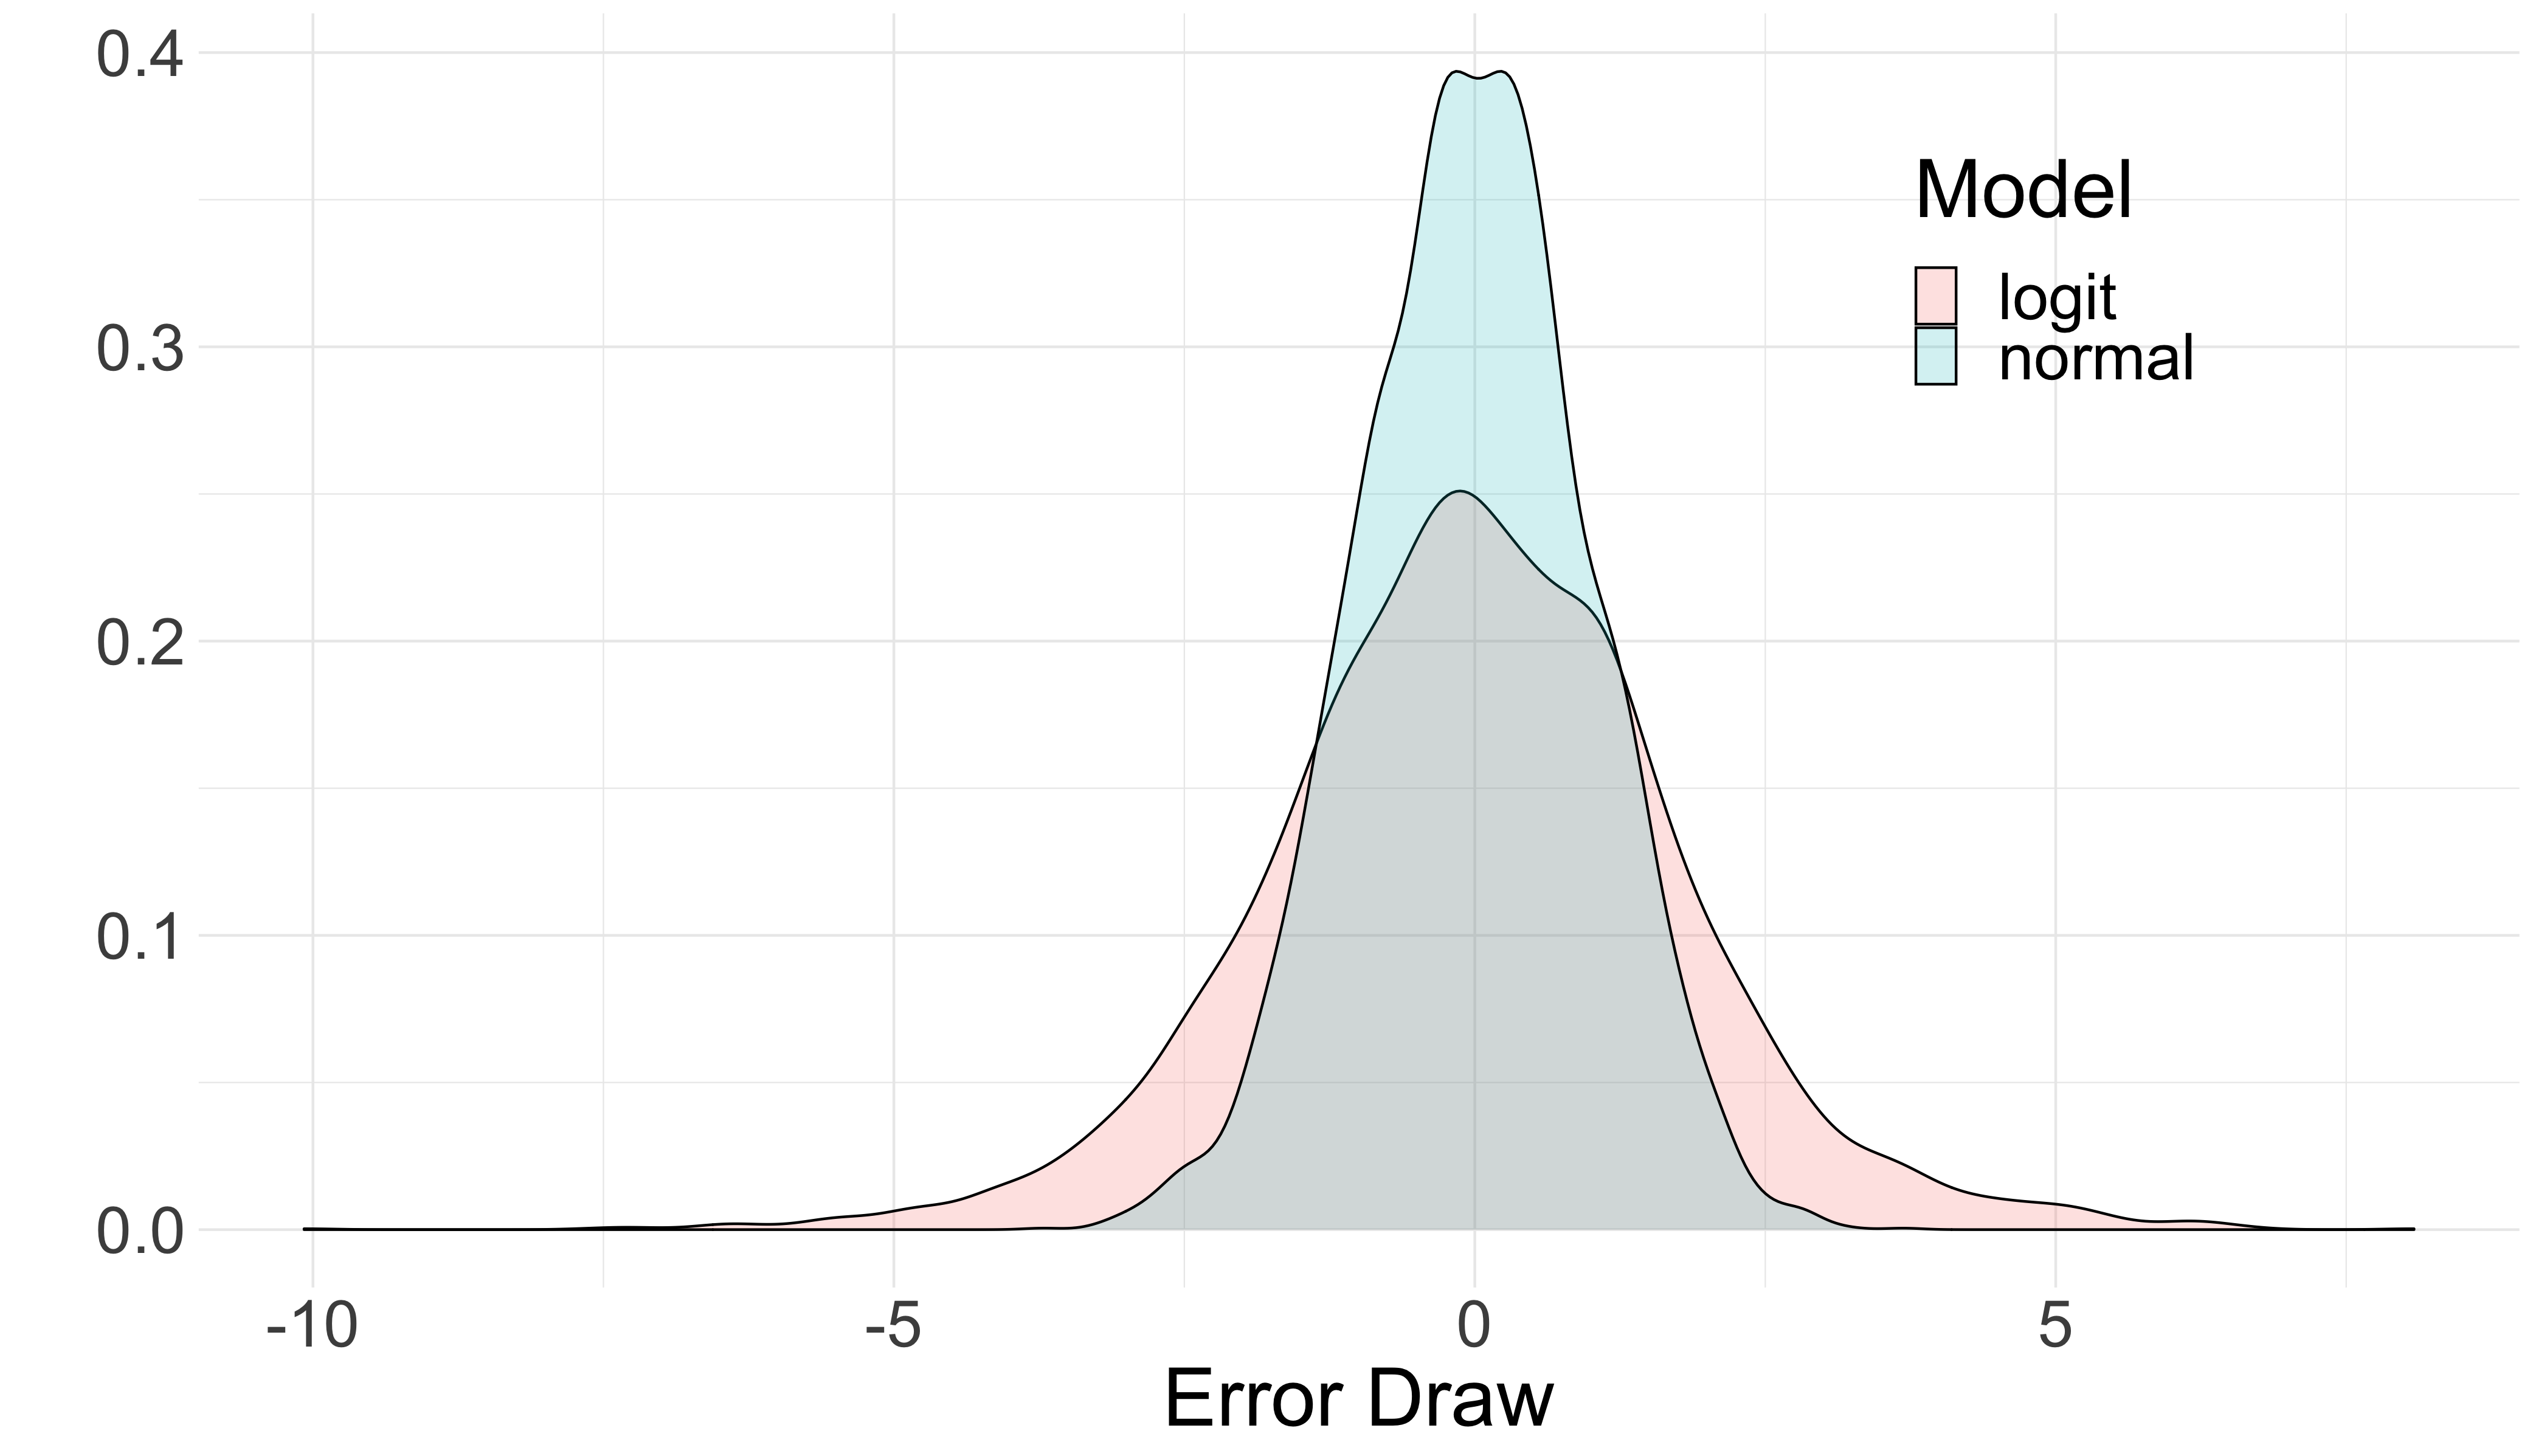
\includegraphics[width=\linewidth]{../lectures/images/logit_v_normal.png}
\end{marginfigure}

Note that these are not, in the binary setting, deeply substantive assumptions. In \Cref{fig:logit_v_normal}, we see that there are very minor differences in the thickness of the tails for a logit vs. normal error, but they're both symmetric and centered around zero.\footnote{Important caveat: these models only identify $\beta$  up to scale.  Why?  The ``true'' model of $\epsilon$ could have variance  $\sigma^{2}$ that is unknown. 
Consider if $F(X_{i}\beta) = \Phi(X_{i}\beta)$. If this were a general normal (rather than standardized with variance 1), we could just scale up the coefficients proportionate to $\sigma$ and the realized binary outcome would identical.  Hence, we normalize $\sigma = 1$ in most cases. This is \emph{not} a meaningful assumption.} One downside for probit models is that there's no closed form solution for $\Phi$, the CDF for the normal distribution:
\begin{equation}   
    \Phi(X_{i}\beta) = \frac{1}{\sqrt{2\pi}}\int_{-\infty}^{X_{i}\beta}e^{-t^{2}/2}dt
\end{equation}

We will discuss later how to estimate $\beta$ given these assumptions, but they will involve numerical optimization, as there is no closed form for $\beta$ like in linear regression.

\begin{margintable}
    \caption{Homeownership problem estimated with logit}
    \label{tab:logit_homeowner}
    \begin{tabular}{lrrr}
        & (1) & (2) & (3) \\
      term  &      logit est. & linear est. & avg. deriv. \\
      \midrule
      constant &      -2.14      &        0.0242 & -0.392 \\
      age      &         0.0903  &          0.022& 0.0166\\
      age$^{2}$ &          -0.0006&         -0.0002 & -0.0001\\
      income/10k     &       0.0716       &     0.0069 & 0.0131  
    \end{tabular}
\end{margintable}
\begin{boxD}
    \begin{continueexample}{example:homeownership}
        Consider now the same homeowner problem from \Cref{example:homeownership}, but estimated with logit.  The $\beta$ coefficients in Column 1 of \Cref{tab:logit_homeowner} are hard to interpret. To see why, consider the derviative of the probability with respect to $X_{i}$: 
         \begin{align*}
            \frac{\partial Pr(Y_{i} = 1 | X_{i})}{\partial X_{i}} &= \beta\phi(X_{i}\beta) &\qquad \text{(Probit)}\\
            \frac{\partial Pr(Y_{i} = 1 | X_{i})}{\partial X_{i}} &= \beta \frac{\exp(X_{i}\beta)}{(1+\exp(X_{i}\beta))^{2}}  &\qquad \text{(Logit)}.
         \end{align*}
        In both cases, the effect of $X_{i}$ changes, depending on the value of $X_{i}$. This is a problem for interpretation.  The average derivative in Column 3 is a way to get around this, but it's not a perfect solution:
        \begin{align*}
        n^{-1}\sum_{i} \frac{\partial E(Y|X)}{\partial X} 
        &=n^{-1}\sum_{i} \beta \frac{\exp(X_{i}\beta)}{(1+\exp(X_{i}\beta))^{2}}
        \end{align*}
        This will calculate the derivative for every value in the sample, and then average them.  This is a way to get a sense of the average effect of $X_{i}$ on $Y_{i}$. We see a much larger effect of income on homeownership in the logit model than in the linear model (Column 2).
    \end{continueexample}
\end{boxD}
  
\begin{figure}
    \caption{Linear vs. Logit model predictions}
    \label{fig:linear_v_logit}
    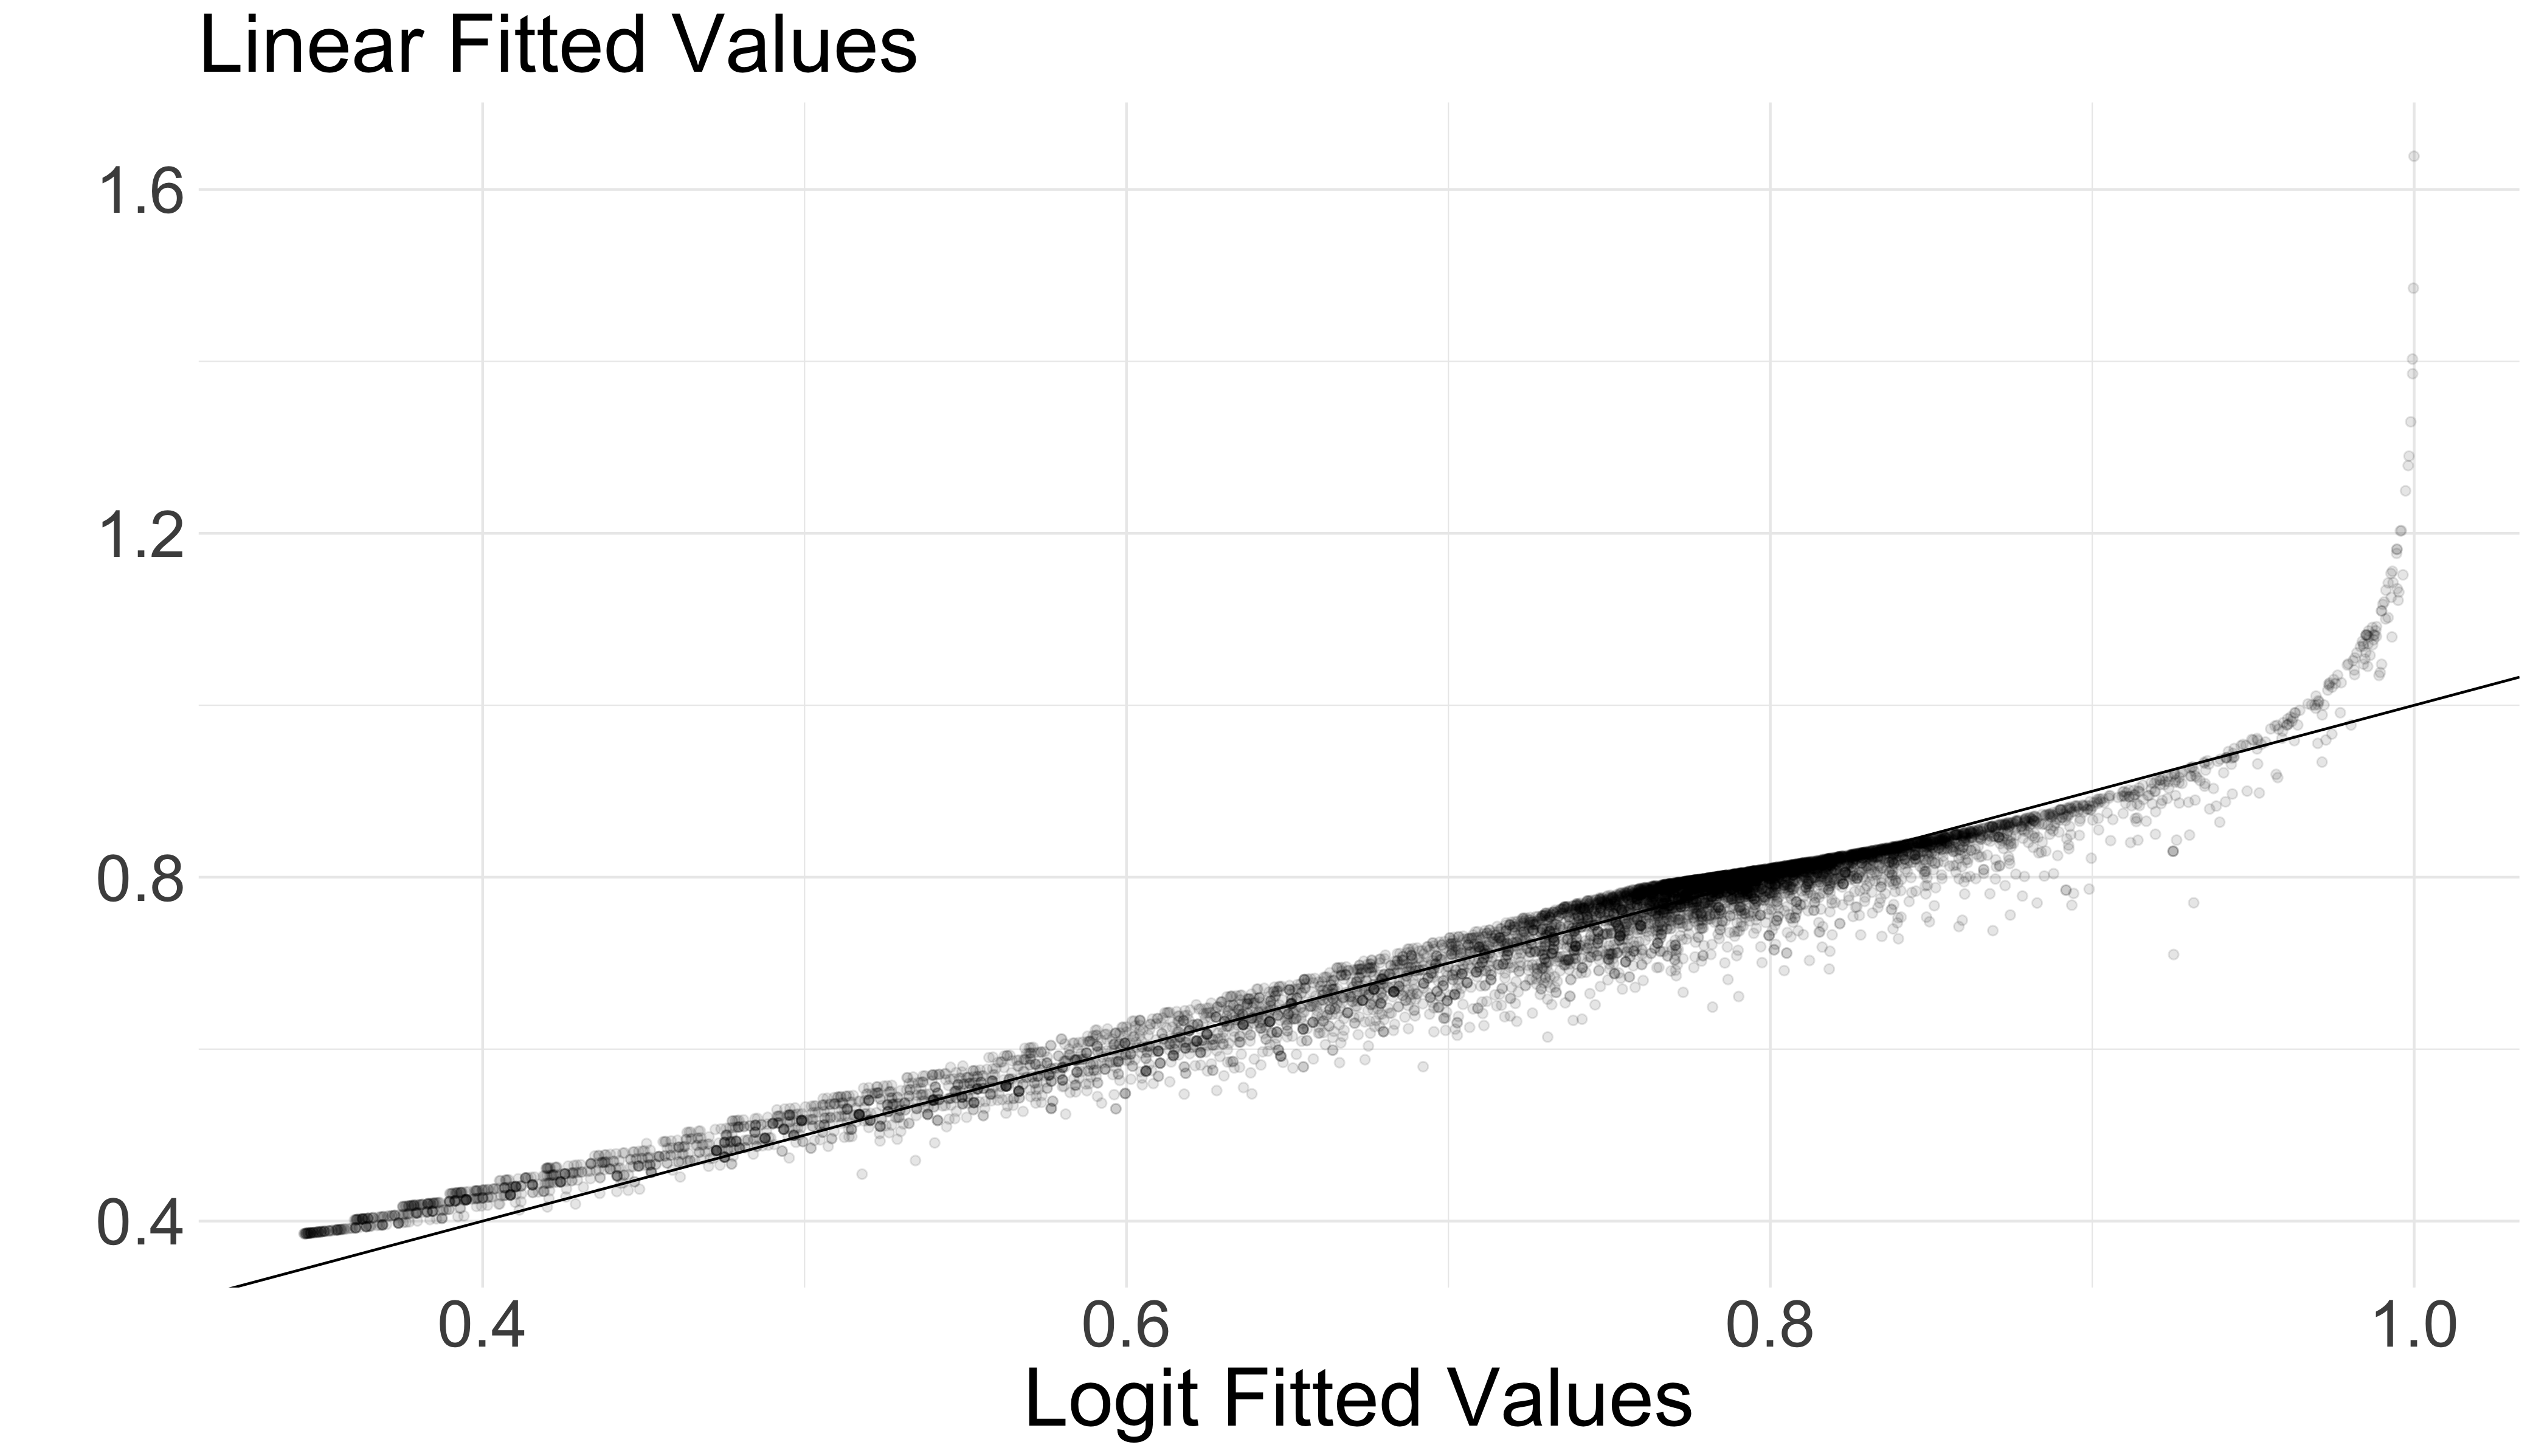
\includegraphics[width=\linewidth]{../lectures/images/linear_v_logit_scatter.png}
    \end{figure}
  
\begin{boxD}
    \begin{continueexample}{example:homeownership}
        \Cref{fig:linear_v_logit} shows the predicted values of homeownership from the linear and logit models.  The linear model is predicting values outside of the support of the outcome, and the logit model is not.  This is one benefit of correctly specifying the model. 
    \end{continueexample}
\end{boxD}
  
\section{Generalized Linear Models (GLM)}
We can generalize the intuition above, where we let the underlying distribution of $\epsilon$ be non-normal, and parameterize the mean of the distribution to be a function of $X_{i}\beta$. This is the idea behind Generalized Linear Models (GLM), originally formulated in \citet{nelder1972generalized}.\footnote{Interestingly, this is very common in non-economics fields, but much less common in economics.} 

The overall setup of GLMs in broad strokes is to consider estimation of a \textbf{linear model $X\beta$}, which is linked to the conditional mean $E(Y|X)$ by \textbf{a link function $g$}: $E(Y|X) = g^{-1}(X\beta)$. The crucial underlying machinery is based on the idea that $Y$, the outcome, is distributed by some member of the \textbf{exponential family} of distributions. This includes the normal, binomial, Poisson, and gamma distributions, among others. Quite notably, though, as we discuss below, this distribution does not have to be correctly specified for the parameter estimates for the conditional mean to be consistent.

Some simple examples of GLMs include:
        \begin{enumerate}
        \item Logit, with a link function $g^{-1}(X_{i}\beta) = \frac{\exp(X_{i}\beta)}{1+\exp(X_{i}\beta)}$
        \item Normal, with an identity link function $g^{-1}(X_{i}\beta) = X_{i}\beta$
        \item Poisson, with a log link function $g^{-1}(X_{i}\beta) = \exp(X_{i}\beta)$
        \end{enumerate}

In essence, we can enforce a linear functional form to the \emph{mean}, and allow the error distribution to fit the form of the data.\footnote{It's interesting to note the underlying machinery of GLMs is similar to many of the selection and discrete choice models we've discussed and discuss today. The linear index provides an extremely convenient parameterization of the mean, but also makes some particular assumptions about the substitutibilty of the covariates.} 

We will now discuss the Poisson regression case in more detail, as it tends to be underused in economics, and is a very important use case. A key takeaway in GLM, like with OLS, is that it is possible to correctly specify just the conditional mean function and then robustly estimation standard errors on parameters of that function, rather than fully specifying the distribution correctly.

\subsection{Poisson Regression for non-negative outcomes}

Consider an non-negative outcome $Y \geq 0$. There are a huge host of outcomes in economics and finance that are restricted to this support: investment, assets, wages, patent citations, output, and so on. We are often interested in the estimand of the partial effect $dE(Y | X) / dX$. If we estimate this conditional with linear regression (e.g. by assuming $Y_{i} = X_{i}\beta + \epsilon_{i}$), what are potential issues?

Mechanically, the error terms $\hat{\epsilon}_{i} = Y_{i} - X_{i}\hat{\beta}$ will be skewed, since $Y_{i}$ is skewed. This is not on its own a huge issue, but it does suggest that the asymptotic approximation for $\hat{\beta}$ will be worse for a given $n$. This leads to highly influential outliers for OLS as well.\footnote{Note that one solution to this issue is to consider quantile regression instead!} 


\begin{boxF}
\begin{cmt}
  Consider two outcomes, $Y_{1}$ and $Y_{2}$. In both cases, the true model is linear (with coefficient of 1) with respect to $X$, but the error term is Normal with mean zero and variance 1 in $Y_{1}$, and is log-Normal with mean zero and variance 1 in $Y_{2}$. If we simulate and estimate this model using linear regression, plotting the t-statistic of the coefficient on $X$ for each model, we find much higher power for the model with Normal errors, rather than log-Normal errors. This reflects the lack of efficiency of OLS in the presence of non-Normal errors (but not a lack of consistency!). See \Cref{fig:non_normal_errors} for a visual representation of this.
\end{cmt}
\end{boxF}

\begin{marginfigure}
  \caption{Non-normal errors in linear regression}
  \label{fig:non_normal_errors}
  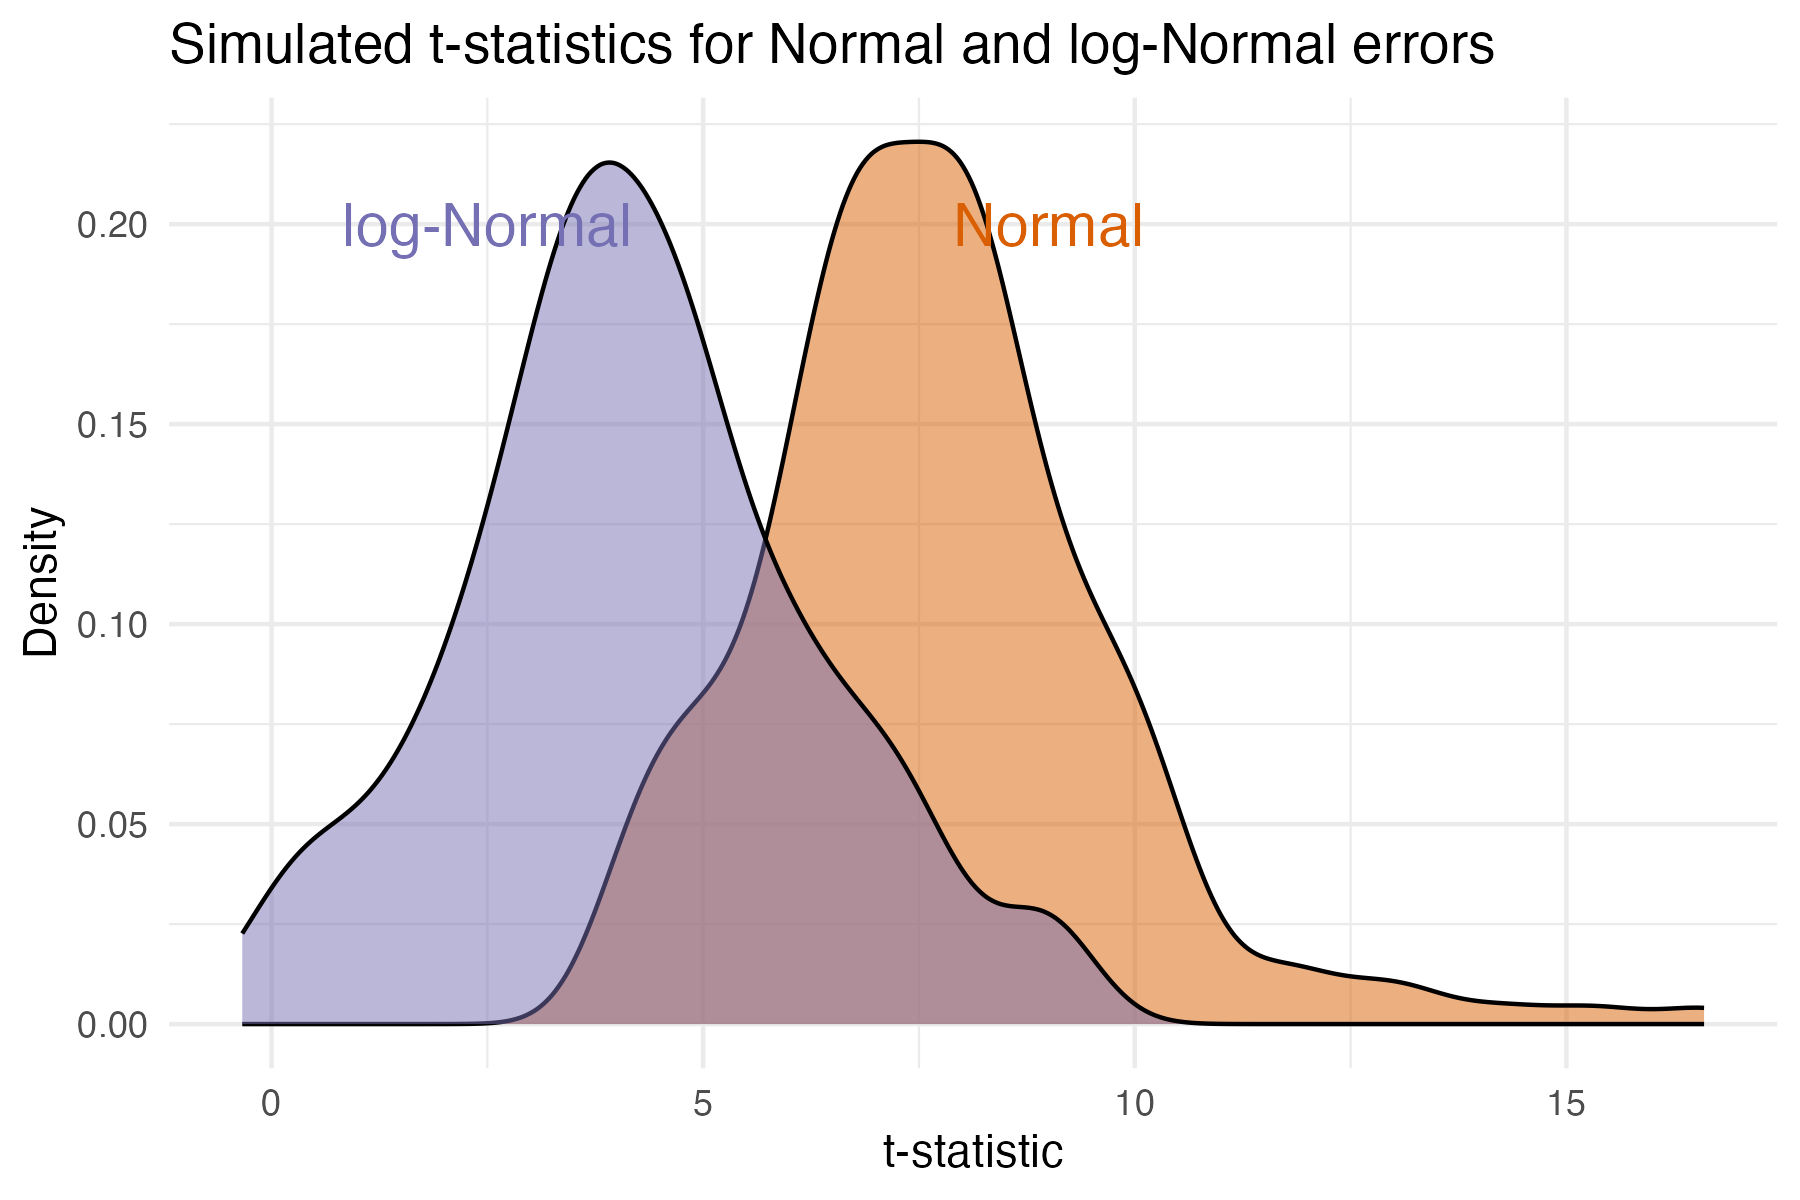
\includegraphics[width=\linewidth]{note_code_9.png}
\end{marginfigure}

What are solutions to this issue? One commonly used approach is to estimate linear regressions on $\log(Y)$ instead of $Y_{i}$. This solves many of the outlier and skew issues,\footnote{In the ideal case, note that a log-Normal outcome will be exactly linear after using logs.} but creates its own problems. 

First, the parameters have a different interpretation. Note that the units for the outcome are different (log points). Often, these are interpreted in percentage points, since log differences are approximately equal to percentage changes.\footnote{Recall $\log(Y_{1}) - \log(Y_{0}) = \log(Y_{1}/Y_{0}) = \log(1+\Delta Y / Y_{0}) \approx \Delta Y / Y_{0}$ for $\Delta Y / Y_{0}$ small.  } This is useful, but can at times be confusing (e.g. what is the actual level effect? Sometimes a percentage effect can exaggerate or minimize a large level effect). 

Second, what if $Y = 0$? This is a problem, as $\log(0)$ is undefined. One common solution is to use $\log(1+Y)$ or $arcsinh(Y)$ \citep{MANNING2001461, ravallion2017concave, bellemare2020elasticities}, which solves the second problem, but makes the first problem even worse! \citep{ bellemare2020elasticities, aihounton2021units, cohn2022count} Why these solutions? For one, they're both well-defined at $Y=0$. Second, it has ``similar'' properties to the taking a log. Effectively, since the distance between $\log(1+Y)$ and $\log(Y)$ was small as $Y$ gets large, the hope is that the differences would ``wash out.''  It turns out, thanks to work by \citet{chen2023logs}, that neither of these solutions are a good idea and that these differences do not wash out.

The key point of \citet{chen2023logs} is that percentage effects are not well-defined for outcomes that are potentially zero-valued. That is in some ways obvious -- there is no way to talk about the percent increase for something where the base-level is zero. Dividing by zero is infinite! But recall that part of the goal of using log outcomes was to approximate percentage changes in the outcome due to treatments. The main result of \citet{chen2023logs} shows that for \emph{any other function} approximating $\log$, but defined at zero, the results will be arbitrarily sensitive to changes in units (e.g. dollars to yuan).\footnote{This includes both $\log(1+y)$ and $arcsinh(y)$.}  

What drives this effect? Effects close to zero and at zero. Most importantly, the \emph{extensive margin} of moving from zero to non-zero has huge, and arbitrary, impacts on estimates on these types of rescaling. Put precisely, if you change the units of the outcome by $a$ (e.g. $a=100$, converting from cents to dollars), then the estimated effect will change by $\log(a)$ multiplied by the \emph{extensive margin} effect. Note that this is fails scale equivariance, which is the property of OLS and quantile regression that usually makes a good estimator.\footnote{Note also the practical implication: if there is a big extensive margin effect, a large $a$ has a big effect. In contrast, with a small $a$, then most effects will be close to zero (since they are extensive margin, and hence close to zero by definition).} 

This can have some really serious implications. \citet{chen2023logs} find that for half the papers they surveyed in the AER, the estimated effects would change by more than 100\% if the units of the outcome were changed by 100 (e.g. dollars to Yen). This is a non-trivial effect! 

The takeaway I want you to have: you should not be running a regression with $\log(1+Y)$ or $arcsinh(Y)$ on the left-hand side!\footnote{I have done this, historically, in my own work -- we're all flawed creatures trying to inch towards better methodological implementations!} So what should you do if you have a zero in your left-hand side variable? \citet{chen2023logs} suggest other ways of considering these situations:\footnote{These solutions are not perfect, but are motivated by a ``trilemma'' they prove: it is not possible to have an estimator that is simultaneously (1) an average of individual level treatment effects (2) invariant to rescaling of units and (3) point-identified without more assumptions about the joint distribution of the potential outcomes (beyond what we usually do in regression).}
\begin{enumerate}
  \item First, if you really need something interpretable as as a percentage effect (e.g. rescaling an ATE into percentage), you could estimate $\tau = E(Y_{i}(1) - Y_{i}(0)) / E(Y_{i}(0))$, which scales the ATE by the baseline average. \emph{This is the estimand targeted by Poisson regression.} There are also other normalizations one could consider. Instead of normalizing by $E(Y_{i}(0))$, if there is a pre-treamtent characteristic that is exogeneous, you could normalize by $E(Y_{i}(0) | W_{i})$, e.g. the predicted baseline value given characteristic $W_{i}$. This captures richer heterogeneity in the baseline characteristic, and may do a better job of reducing skewness. 
  \item Second, you could redefine the outcome in terms of functionals of the distribution, e.g. $\tilde{Y} = F_{Y^{*}}(Y)$. A prominent example is looking at the rank of an individual relative to the overall individual, as in \citet{chetty2014land}. 
  \item If the goal is to consider trade-offs in some like concave preferences, then it is plausible to specify exactly the 'value' of a person at $Y = 0$, relative to positive $Y$, and then explicitly evaluate the parameter that way. This has the problem of losing scale-invariance, but at least the research is explicit about how they value these issues.
  \item Finally, it is plausible to directly estimate the extensive and intensive effects separately. However, the intensive effect is only partially identified; we will explore this further in later lecutres. 
\end{enumerate}
See \Cref{tab:chenroth} for a full set of alternative estimators. 
\renewcommand{\arraystretch}{1.2}
\begin{table*}[ht]
  \centering
  \makebox[\textwidth]{ \begin{tabular}{p{3cm}lp{5cm}}
\toprule
  \textbf{Description} & \textbf{Parameter} & \textbf{Pros/Cons} \\ 
  \midrule
  Normalized ATE & $E(Y(1) - E(Y(0))$ & Pro: Percent interpretation \newline Con: Does not capture decreasing returns \\ 
  Normalized outcome & $E(Y(1) / X - Y(0) / X)$ & Pro: Per-unit-X interpretation \newline Con: Need to find sensible X \\ 
  Explicit tradeoff of intensive/extensive margins & \newline 
  $ATE \text{ for } m(y) = \begin{cases}
    \log(y) & y > 0 \\
     -x & y = 0 \\
  \end{cases}$ &  Pro: Explicit tradeoff of two margins \newline Con: Need to choose \(x\); Monotone only if support excludes \( (0, e^{-x}) \) \\ 
  Intensive margin effect & $E \left[ \log \left( \frac{Y(1)}{Y(0)} \right) | Y(1) > 0, Y(0) > 0 \right]$ & Pro: ATE in logs for the intensive margin \newline Con: Partially identified \\
  \bottomrule
  \end{tabular}}
  \caption{Table 2 from Chen and Roth (2023)}
  \label{tab:chenroth}
  \end{table*}

  \begin{boxF}
\begin{cmt}[Poisson Regression]
  Poisson regression is a good example of a way to estimate $E(Y_{i}(1) - Y_{i}(0)) / E(Y_{i}(0))$. This approach estimates $\log(E(Y|X)) = X\beta$, rather than $E(\log(Y)|X)$. You get a simple semi-elasticity measure for the parameters, and $Y$ can be zero. What are the typical concerns?
        \begin{enumerate}
        \item       If $Y | X$ is truly distributed
        Poisson, conditional on $X$, then $Var(Y|X) = E(Y|X)$. This just comes from the Poisson
        distribution's statistical properties, but feels like a restrictive model assumption. But, it's not relevant for the parameter estimates of $\beta$. The estimates are still consistent, and the standard errors for these estimates can be adjusted for misspecification using robust standard errors (e.g. sandwich covariance estimators). These will give correct coverage, obviating any concerns about the Poisson regression. It is \emph{not} necessary to use a Negative Binomial regression.
      \item As we will discuss shortly, in many non-linear models, if you include parameters, such as fixed effects, which cannot be consisitently estimated, then this will make \emph{all} the estimates in the model inconsistent. This is different from linear models. This concern is less of an issue in Poisson regression, as fixed effects can be concentrated out (see \texttt{PPMLHDFE} in Stata and \texttt{glmhdfe} in R)
      \item Individuals are often not sure how to do instrumental variables in Poisson regression, but it is feasible! See \citet{mullahy1997instrumental, windmeijer1997endogeneity}.
      \end{enumerate}

  
The benefits of using the Poisson model (instead of log(1+$Y$)) according to \citet{cohn2022count}:
``We replicate data sets from six papers published in top finance journals that together study two count or count-like outcomes... We...estimate log1plus and Poisson regressions based on that specification, and compare the coefficients of interest. These coefficients differ markedly in all six cases and have different signs in three of the six, suggesting that inference about even the direction of a relationship is sensitive to regression model choice in real-world applications...in all five cases involving regressions with control variables, switching from a log1plus to Poisson regression results in a larger change in the coefficient of interest than omitting the most important control variable, generally by a wide margin.''
    \end{cmt}
  \end{boxF}
  

\subsection{Inconsistency in binary choice models}
Consider estimating a panel fixed effects model with binary choice:
 \begin{align*}
 Y_{it} &= \alpha_{i} + X_{it}\beta + \epsilon_{it}\\
 Y_{it} &= F(\alpha_{i} + X_{it}\beta)
 \end{align*}
 where we are interested in the parameter $\beta$. If we have a short panel (e.g. few time periods), we cannot consistently estimate $\alpha_{i}$. However, in the linear case, this does not affect estimation of $\beta$. More shockingly, however, is that for binary outcome case, the only model that consistently estimates $\beta$ is a conditional Logit \citep{chamberlain1980analysis, chamberlain2010binary}. 
 
More generally, if you have inconsistent fixed effects in your non-linear models, this can cause serious issues (except in special cases like conditional). Often, the only way to get around these issues is by finding ways to ``concentrate'' or get around these nuisance parameters. Famous cases where this occurs include conditional logit, Poisson unit fixed effects, and partial likelihoods in the Cox proportional hazard model. 

% \section{Estimation procedures}
%  How do we estimate these types of problems? Consider the likelihood function for logit:
%       \begin{align*}
%         Pr(Y_{i} = 1 | X_{i} ) &= \frac{\exp(X_{i}\beta)}{1+\exp(X_{i}\beta)}\\
%         l(\beta|\mathbf{Y}, \mathbf{X}) &= \Pi_{i=1}^{n} Pr(Y_{i} = 1 | X_{i} )^{Y_{i}}(1-Pr(Y_{i} = 1 | X_{i} )^{1-Y_{i}}\\
%         L(\beta|\mathbf{Y}, \mathbf{X}) &= \sum_{i=1}^{n} Y_{i}\log(Pr(Y_{i} = 1 | X_{i} ))\\
%                                &+  (1-Y_{i})\log(1-Pr(Y_{i} = 1 | X_{i} ))
%       \end{align*}
% Rule of thumb: the likelihood is the joint probability of the data
%       \begin{itemize}
%       \item We are exploiting the independent nature of the data
%       \item Joint probability of two independent values is the product
%         of their marginals
%       \end{itemize}
% Recall that we can take the log of the likelihood when
%       considering extremes of the function because any maximum will be
%       identical irrespective of monotone transformations
% Plug in Logit to the MLE

% With some simple rewriting:
%       \begin{align*}
%         L(\beta|\mathbf{Y}, \mathbf{X}) &= \sum_{i=1}^{n} Y_{i}\log(\frac{\exp(X_{i}\beta)}{1+\exp(X_{i}\beta)} +  (1-Y_{i})\log(\frac{1}{1+\exp(X_{i}\beta)})\\
%         &= \sum_{i=1}^{n} Y_{i}X_{i}\beta - Y_{i}\log(1+\exp(X_{i}\beta)) +  (1-Y_{i})\log(1+\exp(X_{i}\beta)))\\
%         &= \sum_{i=1}^{n} Y_{i}X_{i}\beta - \log(1+\exp(X_{i}\beta))
%       \end{align*}
  
%       Great, so how would one estimate this? We have a likelihood, we want to maximize it!
  
% Take derivatives and find the maximum!
%         \begin{itemize}
%         \item Finally that calculus is paying off!
%         \end{itemize}
  
% Good news and bad news. There's no analytic solution for this $\beta$. Unlike with OLS, we
%       can't get a closed-form solution for our estimate -- this is true
%       of most estimators. In fact, this is a well-behaved problem,
%       relative to most.
%       \begin{itemize}
%       \item Well-behaved because it's globally concave and has easily
%         calculated first and second derivative
        
%       \end{itemize}
%   So,  What's the good news? We have computers!
  
%  While there is not an analytic solution, if there is a
%         maximum where $\hat{\beta}$ satisfies
%         $\frac{\partial L(\hat{\beta})}{\partial \beta} = 0$, then there
%         are sets of conditions such that
%         \begin{itemize}
%         \item $\lim_{n\to\infty}\Pr(||\hat{\beta}_{n} - \beta_{0}|| > \epsilon) = 0$ (weak consistency)
%         \item $\lim_{n\to\infty} \sqrt{n} (\hat{\beta}_{n} - \beta_{0}) \rightarrow^{d} \mathcal{N}\left(0, -E\left[\frac{\partial^{2}}{\partial\beta \beta'}L(\beta_{0})\right]\right)$ (asymptotic normality)
%         \end{itemize}
% The challenge is that the conditions for when this is
%         satisfied vary from problem to problem
% Most general results in this put high-level assumptions on
%         the problem, and then the conditions need to be checked
   
  
% While there is not an analytic solution, if there is a
%         maximum where $\hat{\beta}$ satisfies
%         $\frac{\partial L(\hat{\beta})}{\partial \beta} = 0$, then there
%         are sets of conditions such that
%         \begin{itemize}
%         \item $\lim_{n\to\infty}\Pr(||\hat{\beta}_{n} - \beta_{0}|| > \epsilon) = 0$ (weak consistency)
%         \item $\lim_{n\to\infty} \sqrt{n} (\hat{\beta}_{n} - \beta_{0}) \rightarrow^{d} \mathcal{N}\left(0, -E\left[\frac{\partial^{2}}{\partial\beta \beta'}L(\beta_{0})\right]\right)$ (asymptotic normality)
%         \end{itemize}
% he conditions for when this is satisfied vary from problem
%         to problem
%  Most general results in this put high-level assumptions on
%         the problem, and then the conditions need to be checked for a particular problem
%         \begin{itemize}
%         \item These general types of problems are classified into $M$-estimation
%           and $Z$-estimation
%         \item $M$-estimation is a general problem where $\beta_{0} = \arg\max_{\beta} E(m(\beta))$
%         \item $Z$-estimation $\subset$ $M$-estimation focused on
%           exploiting features of the derivative of $m(\beta)$
%         \end{itemize}
  
% \section{Numerical optimization}
% In our applications, very well-defined solutions. We'll
%         instead focus on the actual computation of these maxima

%         There are many numerical optimization methods. I'll outline
%         info on the few I know, but this is in no way exhaustive
      
%         A common simple method is Newton-Raphson
  
%   \subsection{Newton-Raphson}   
% Let $Q(\theta) = -L(\theta)$ (denote with $\theta$ to
%         highlight that this is a general problem)
% Idea is to take some arbitrary objective function and fit a
%         local quadratic based on derivatives
%         \begin{itemize}
%         \item Find the minimum based on this quadratic
%         \item Take that minimizer and repeat
%         \end{itemize}
% Specifically, let
%         $$ \theta_{k+1} = \theta_{k} - \left[\frac{\partial^{2}Q(\theta_{k})}{\partial\theta \partial \theta'}\right]^{-1}\frac{\partial Q}{\partial \theta}(\theta_{k})$$
% In our Logit application, we already know the first derivative -- calculating the second derivative is straightforward. Hence, we can solve for $\theta$
%         \begin{itemize}
%         \item We benefit from a convex problem and an easily defined second derivative
%         \end{itemize}
  
% What if we don't know our second derivative? (or it is onerous to
%       calculate)
% Then we can reframe to the problem in two pieces.  Let $A_{k}$ be
%       any positive definite matrix. Consider the following iterated estimation:
%       $$ \theta_{k+1} = \theta_{k} - \lambda_{k}A_{k}\frac{\partial Q}{\partial\theta}(\theta_{k})$$
  
% This nests Newton-Raphson:
%       \begin{itemize}
%       \item $\lambda_{k} = 1$
%       \item $A_{k} = \left[\frac{\partial^{2}}{\partial\theta \theta}L(\theta_{k})\right]^{-1}$
%       \end{itemize}
  
%   Intuitively, there are two pieces:
%       \begin{itemize}
%       \item  a steplength (defined by $\lambda_{k}$)
%       \item a direction
%         $d_{k} = A_{k}\frac{\partial Q}{\partial\theta}(\theta_{k})$
%         (controlled by $A_{k}$, which select a direction of the
%         gradient)
%         \begin{itemize}
%         \item A convenient rescaling is $\tilde{d}_{k} = d_{k} / (1 + \sqrt{d_{k}'d_{k}}$ to ensure $|\tilde{d}_{k}| < 1$
%         \end{itemize}
%       \end{itemize}
  
% We can choose the direction, then choose how far we want to go
        
% \begin{equation}
%     \lambda_{k} = \arg\min_{\lambda}Q(\theta_{k} + \lambda \tilde{d}_{k})  
% \end{equation}
% Simplest version verison of this is $A_{k} = I_{k}$        (identity matrix) -- just go in the direction of steepest
%         descent. How does one calculate $\lambda_{k}$ in these settings? If $\theta$ is scalar, it's feasible (but inefficient) to calculate
%         using a simple grid search. In high-dimensions, too slow (and our next algorithm needs
%         optimal choice to converge)
  
% Two line search algorithms
%  Newton's Method
 
%  Given a $d$, recall we need a $\lambda$. Redefine $\lambda^{*} = \arg\min_{\lambda} Q(\lambda)$
% The simplest method is Newton's method (which finds the root
%         of a function (we want the root of the derivative)
%  Begin with an initial guess for $\lambda_{0}$. Then,
%         $$\lambda_{k+1} = \lambda_{k} - \frac{Q'(\lambda_{k})}{Q''(\lambda_{k})}$$

%         Repeat till $|\lambda_{k+1}-\lambda_{k}|$ is small
%         (e.g. convergence)
%  Issue with this approach is you need a second derivative

%   Golden Search
 
%  Start with two points you know for certain contain the minimum (need unimodality)
%         \begin{itemize}
%         \item E.g. $\lambda_{l} = 0, \lambda_{h} =
%           1$ [Picking an abritraily large $\lambda_{h}$ is fine -- there
%           are ways to check this]
%         \end{itemize}

%         Two points on the line segment between: $\lambda_{m1} = \lambda_{l} + 0.392 \times (\lambda_{h} - \lambda_{l})$ and $\lambda_{m2} = \lambda_{l} + 0.618 \times (\lambda_{h} - \lambda_{l})$

%         Now, given the three segments, can check two conditions:
%         \begin{itemize}
%         \item $Q(\lambda_{m2}) > Q(\lambda_{m1})$: you know that the minimizing value of  $\lambda $ in [$\lambda_{l}$, $\lambda_{m2}$]. Update your values:  $\lambda_{l}' = \lambda_{l}$, $\lambda_{h}' = \lambda_{m2}$, $\lambda_{m2}' = \lambda_{m1}$, $\lambda_{m1}' =  \lambda_{l}' + (\lambda'_{h} - \lambda'_{m2}$
%         \item $Q(\lambda_{m2}) < Q(\lambda_{m1})$: you know that the minimizing value of  $\lambda $ in [$\lambda_{m1}$, $\lambda_{h}$]. Update your values:  $\lambda_{h}' = \lambda_{h}$, $\lambda_{l}' = \lambda_{m1}$, $\lambda_{m1}' = \lambda_{m2}$, $\lambda_{m2}' =  \lambda_{h}' - (\lambda'_{m1} - \lambda'_{l}$
%         \end{itemize}
% Update until you find the optimal $\lambda$

% Davidson-Fletcher-Powell (DFP) is more elaborate, and requires all these pieces
%         \begin{itemize}
%         \item Commonly used, although not the fastest algorithm out there now
%         \end{itemize}
% Its strongest feature is that it is efficient and can work
%         without calculating a second derivative

% Initiate with any positive definite matrix $A$
%         (e.g. identity matrix)
% Steps (repeat till convergence):
%         \begin{enumerate}
%         \item Calculate direction $\tilde{d}_{k}$
%         \item Calculate optimal step length $\lambda_{k}$
%         \item Calculate the actual step
%           $p_{k} = \lambda_{k}\tilde{d}_{k}$ and the new parameter
%           $\theta_{k+1} = \theta_{k}+ p_{k}$
%         \item Calculate the change in the derivative $q_{k}$ from
%           $\theta_{k}$ to $\theta_{k+1}$
%         \item Update
%           $$A_{k+1} = A_{k} + \frac{p_{k}p_{k}'}{p_{k}'q_{k+1}} - \frac{A_{k}q_{k+1}q_{k+1}'A_{k}}{q_{k+1}'A_{k}q_{k+1}}$$
%         \end{enumerate}

\section{Multiple Choices}
 We'll now examine multiple discrete choice problems. Much of this discussion is very adjacent to industrial organization. However, many of these ideas are important for non-IO problems, such as multiple IVs and Roy models. Moreover, these tools are very promising in fields that  have not yet used them.
 
 Issues with choice problems that we'll discuss:
\begin{itemize}
\item Independence of Irrelevant Alternatives (IIA)
\item Choice sets and consideration sets
\end{itemize}
      
Consider the following problem: we observe choices for individuals $Y_{i} = j$, $j \in \Omega = \{0, 1, \ldots, J\}$, where $J+1 = |\Omega|$ is the total number of choices.  Importantly, the order of the choices has no particular meaning. This could be red bus, blue bus and car as transportation choices, for example. 

Given these sets of choices, we have different types of covariates we can observe. Some characteristics are choice specific (such as a price), while some are unit specific (such as a person's income). Often, we want to allow for the characteristics to vary by both dimensions. This includes allowing for a choice's characteristic to vary depending on the person (e.g. a unit specific coefficient on the choice's  characteristic), or allowing the person's characteristic to have differential effects on the choice of different goods. In total, we have three types of characteristics:
\begin{enumerate}
\item $X_{i}$ (individual characteristics, invariant to choices),
\item   $X_{j}$ (choice characteristics) 
\item  $X_{ij}$ includes individual-by-choice characteristics
\end{enumerate}
We can write $X_{i}$ as $X_{ij}$ by interacting with choice  fixed effects, and $X_{j}$ can have $i$ speicfic coefficients.\footnote{Note that when $J = 1$, we collapse down to binary choice.}

Now recall there are two (non-exclusive) ways to think the discrete choice problem.  The first is a statistical view: namely, how do we model the choice probabilities? In the binary choice problem, there is only one parameter that needs be known, conditional on $X_{i}$:  $\pi(X_{i}) = Pr(Y_{i} = 1 |X _{i})$  With more than two choices, the dimensionality becomes more complicated.  We now have  $\pi_{j}(\mathbf{X}), j=2,3$ for 3 choices. 

 How should we parameterize how other choices' characteristics affect each other? Most of the models we will discuss will make very specific restrictions on how choices affect one another.  These are not innocuous choices, as we'll see, but they provide a huge amount of additional structure that can be used to identify the parameters of interest.
      
\subsection{The naive approach}

If we want to estimate simple treatment effects, we could focus on binary outcomes. For exmaple: we have a randomly assigned treatment $T$, and $J$ choices. What is the effect of $T$ on $Pr(Y_{i} = j)$ under random assignment?
 \begin{equation}
    \tau_{j} = Pr(Y_{i} = j | T_{i} = 1) -Pr(Y_{i} = j | T_{i} = 0)
 \end{equation}
 The downisde of this approach is that there's no information about the substitution patterns of individuals in this form. Concretely, if $\tau_{2}$ is positive, is that because the share of individuals choosing $Y_{i} = 1$ decreases,  the share of individuals choosing $Y_{i} = 0$ decreases, or both?  Namely, what is the \emph{substitution} pattern across the choices?\footnote{To put a statistical note on this, there are effectively two endogenous variables ($1(Y_{i} = 1) $ and $1(Y_{i} =2)$), and we only have one randomly assigned variable $(T)$. Hence, there's no way to simultaneously identify the effect on both.} 
 
 Nonetheless, it is still very helpful to estimate these measures, and it's useful when faced with a lot of choices to focus on the effect on one margin. We will need more structure to estimate relative choice substitution across outcomes, and ask questions like ``what is the effect of $T$ on choosing $j$ conditional on choosing $j$ or $k$?''
      
\subsection{Conditional logit}
A second way to view the problem is as an structural (economic) choice problem (pioneered by McFadden \citep{mcfadden1972conditional}). Consider a set of utilities $U_{ij}$ (unobserved) such that 
 
\begin{equation}
  Y_{i} = \arg\max_{j \in \Omega}U_{ij}.
\end{equation}

In other words, person $i$ chooses $j$ if it's the choice that maximizes the utility amongst all $J+1$ choices.   Note the similarity to the $Y^{*}_{i}$ in the binary case!

If we make the assumptions:
\begin{enumerate}
\item  $U_{ij} = X_{ij}'\beta + \varepsilon_{ij}$
\item $\epsilon_{ij}$ are independent across choices and
  individuals, and distributed Type-I extreme value
\end{enumerate}
then we get the McFadden conditional logit model:

\begin{equation}
  \label{eq:mcfadden}
  Pr(Y_{i} = j | X_{i}) = \frac{\exp(X_{ij}\beta)}{\sum_{k=0}^{J}\exp(X_{ik}\beta)}.
\end{equation}

\begin{boxF}
  \begin{cmt}
  Note that if the characteristics $X_{ij}$ only vary based on the individual (e.g. we can write $X_{ij}\beta$ as $X_{i}\beta_{j}$), then the effects across choices are \emph{relative} to each other. We can write our probability equation as
\begin{equation}
  Pr(Y_{i} = j | X_{i}) = \frac{\exp(\alpha_{j} + X_{i}\beta_{j})}{1 + \sum_{k=1}^{J}\exp(\alpha_{k} + X_{i}\beta_{k})}.
\end{equation}
This is the \emph{multinomial logit}. Once we allow for choice speicfic characteristics, then we need to write the probability following \Cref{eq:mcfadden}.
  \end{cmt}
\end{boxF}

In many choice problems, a key parameter we're interested in is the price elasticity. The definition of the price elasticity is the percentage change in a market share of a good for a given percentage change in the price. Formally, the own-price elasticity is:
\begin{equation}
  \epsilon_{j} = \frac{\partial Pr(Y_{i} = j | X_{ij})}{Pr(Y_{i} = j | X_{ij})}\frac{p_{j}}{\partial p_{j}} = \frac{\partial Pr(Y_{i} = j | X_{ij})}{\partial p_{j}}\frac{p_{j}}{Pr(Y_{i} = j | X_{ij})}.
\end{equation}
We can \emph{also} think about \emph{cross}-price elasticities, e.g. how do market shares change when other goods shift their price: 
\begin{equation}
  \epsilon_{jk} = \frac{\partial Pr(Y_{i} = j | X_{ij})}{\partial p_{k}}\frac{p_{k}}{Pr(Y_{i} = j | X_{ij})}.
\end{equation}
Note that with \cref{eq:mcfadden} as our probability model, we can estimate all these elasticities (assumign we have the data on prices, and we are willing to assume prices are exogeneous, a very strong assumption). But, this formulation creates issues.
      
A key issue with this formulation of the conditional logit model is that the cross-price elasticities are identical. Specifically, $\epsilon_{jk} = \epsilon_{lk}$, such that the effect of shifting price of a different good causes an identical proportionate shift in all choices' market share. You can see this by simply plugging in for $ \frac{\partial Pr(Y_{i} = j | X_{ij})}{\partial p_{k}}$:  \begin{align*}
            \epsilon_{jk} &= \underbrace{-\gamma Pr(Y_{i} = j|X_{ij} )Pr(Y_{i} = k | X_{ij} )}_{\frac{\partial Pr(Y_{i} = j | X_{ij} )}{\partial p_{k}}} \times \frac{p_{k}}{Pr(Y_{i} = j | X_{ij})}\\
                          &= -\gamma Pr(Y_{i} = k | X_{ij} )p_{k},
          \end{align*}
where $\gamma$ is the coefficient on price in the conditional logit model. Note that this elasticity is not a function of $j$, and hence identical for all other products.\footnote{It's useful to note that the \emph{levels} of the market share do vary by good, but the elasticity scaling makes the cross-price elasticities identical.} 

The canonical example of this is the ``car, red bus and blue bus'' example. Imagine a choice set where there are three choices for transportation: a car, and two busses: one red, and one blue.  Presumably a person is purely indifferent between red and blue busses. Hence, a shift in the red bus price would presumably cause a bigger substitution from the blue bus than from car users, but the conditional logit (in this form) will not account for this.

How can we deal with the IIA issue? This is a problem of poor substitution patterns, which is an economics problem. In other words, economics  gives us an intuition about the market substitution patterns, and we don't think identical cross-elasticities makes sense. It's also a statistical problem -- there is a very strong statistical functional form we have assummed, which was analytically convenient but has somewhat perverse properties. We will now consider a few (but not all) solutions to the problem proposed in the literature.

\subsection{Data structure}
Before jumping into estimation approaches to improve on the substitition patterns, it is worth touching on the structure of the observed data. Crudely, we can think of there being two types of data we observe. In some cases, we observe the individual's choices, combined with information about the individuals, and the choices themselves.\footnote{Sometimes we even observe their second and third choices, which can be very useful!} Often, these individuals may be in the same market, or in different markets. In other cases, we observe the market shares of the choices, the overall characteristics of the individuals in the market, and the characteristics of the choices.\footnote{Note that we could construct the market shares directly from the individual data, assuming that it's a random sample of the population.}

Note that the market share implied by the model in \Cref{eq:mcfadden} is just $s_{j} \equiv Pr(Y_{i}=j|X_{i})$. We can then think about transformations of this market share: $\log(s_{j}) = X_{ij}\beta - \log(\sum_{k=0}^{J}\exp(X_{ik}\beta))$. 

\subsection{Nested Logit and Correlated Multivariate Probit}

One part of the IIA problem comes from the independence of $\varepsilon$ across choices. Recall that the $\varepsilon$ effectively rationalize the market shares beyond what we observe that is explained based on the covariates. Recall the blue and red bus case: getting two independent $\varepsilon$ draws for the busses is not an intuitive view of bus demand. Instead, the blue and bus likely have highly correlated epsilon draws (if not identical), e.g. the unobserved latent demand for blue and red busses is correlated!  The issue is exactly how to specify the correlation  that preserves the ability to estimate the model.

With the nested Logit approach, you can specify sets (as the researcher), and allow correlation of the $\varepsilon$ within these sets. The key is that the errors are uncorrelated across choice sets, which preserves the logit structure (see \citet{goldberg1995product} for an example application), and the correlation \emph{within} a nest is allowed to be correlated following a distinct similarity parameter. In essense, the similarlity parameter scales up and down the effect of the covariates within a nest: if the similarity is high, then the effect of the covariates is swamped by the random error, and the choices are highly correlated; if the similarity is low, the nest approaches the standard IIA setting. See \citet{wen2001generalized} for a more recent discussion.
    
An alternative approach is to allow the covariance matrix of the error terms to be flexibly estimated by the data using a multivariate normal:

\begin{equation}
  \epsilon_{i} = (\epsilon_{i0},\epsilon_{i1},\ldots, \epsilon_{iJ}) \sim \mathcal{N}(0, \Sigma)
\end{equation}
where the researcher will then directly estimate $\Sigma$.  Unfortunately, this problem gets hard with many choices (parameter space grows at rate $O(J^{2})$).   See \citet{mcculloch2000bayesian} and \citet{geweke2003bayesian} for details and an application in the Bayesian setting, and Train (2009) for simulation discussions in  the frequentist case.

%Add Hull Example eventually
% \begin{boxD}
%   \begin{exmp}[Hull, 2020]

%   \end{exmp}
% \end{boxD}

Rather than directly target the distribution of the $\varepsilon_{ij}$, an alternative approach is to add more richness to the coefficients themselves. By adding more random variation in the loadings, it effectively creates a richer substitution pattern by adding more to the error term.  Consider a slight extension of our previous model, with $\beta_{i}$ varying by individual (in an unobserved way):\footnote{Note that this random variation in preferences is usually viewed as \emph{exogeneous}.}
\begin{align*}
U_{ij} &= X_{ij}\beta_{i} + \varepsilon_{ij}\\
U_{ij} &= X_{ij}\overline{\beta} + \nu_{ij}, \qquad \nu_{ij} = \varepsilon_{ij} + X_{ij}(\beta_{i}-\overline{\beta})
\end{align*}
There are a number of ways to estimate this approach, but notice the key point -- subtitution patterns are more richly modeled (and allowed) due to $\nu_{ij}$ varying by $X_{ij}$. 

\begin{boxD}
  \begin{exmp}[Random coefficients estimation example]
    \label{example:random_coefficients}
    Let $J = 3$, and $X_{j}$ be a scalar (e.g. price).  We assume that
    \begin{equation}
      U_{ij} = X_{j}\beta_{i} + \varepsilon_{ij} \qquad \beta_{i} = (\overline{\beta} + \sigma \nu_{i}), \nu_{i}  \sim \mathcal{N}(0, 1). 
    \end{equation}
      Separate the utility of choosing $j$ into 
      \begin{align}
        U_{ij} &= \mu_{ij}(\overline{\beta})  + X_{j} \sigma \nu_{i} + \varepsilon_{ij}\\
        \mu_{ij} &=  X_{j}\overline{\beta}. 
      \end{align} 

      We can write the probability of choosing $j$ as:
    \begin{align}
      Pr(Y_{i} = j | X, \overline{\beta}, \sigma ) &= \int \frac{\exp(X_{j}\overline{\beta} + X_{j} \sigma \nu_{i})}{\sum_{k=0}^{J}\exp(X_{j}\overline{\beta} + X_{j} \sigma \nu_{i})} \phi(\nu_{i})d\nu_{i}
    \end{align}
    where $\phi(\cdot )$ is the Normal standard normal pdf. 

    This setup is often referred to as a ``mixed logit'' model (in contrast with the more common Berry Levinsohn Pakes approach, which we'll discuss later) \citep{mcfadden2000mixed}. The typical approach for estimating these models involves using Maximum Simulated Likelihood, or Method of Simulated Moments. \citet{mcfadden2000mixed} show that a straightforward approach to estimating this is to simulate the model $S$ times, and then use the simulated data to approximate the integral:
    \begin{equation}
      \hat{E}(Pr(Y_{i} = j | X, \overline{\beta}, \sigma ))= \frac{1}{S}\sum_{s=1}^{S}\frac{\exp(X_{j}\overline{\beta} + X_{j} \sigma \nu_{is})}{\sum_{k=0}^{J}\exp(X_{j}\overline{\beta} + X_{j} \sigma \nu_{is})}.
    \end{equation}
    Then, this probability can be used to form a log-likelihood function, and the model can be estimated using standard optimization techniques for maximizing log-likelihoods.

    Note that an important piece in this setting is micro-level choice data (which we use to form the likelihood), and the lack of any unobserved heterogeneity that creates endogeneity and bias in our estimates. Without an additional error term, there's no need for an instrument here. This is a version of assuming exogeneity conditional on observables. Often, we will only observe \emph{market-level} shares of goods. Then, we'll need many markets in order to have sufficient independent variation to estimate parameters. We will discuss this next.
  \end{exmp}
\end{boxD}
      
The workhorse set of demand estimation models is known as BLP (Berry  Levinsohn Pakes), named after the authors in \citet{berry1995automobile}. This model combines random coefficient estimation with unobserved market-good-level demand heterogeneity that is potentially endogeneous and correlated with price. In other words, not only are individuals allowed to have random (independent) error, but there is a fixed unobserved error in demand for each good. This allows for a highly correlated set of demand choices within a market, and also creates unobserved demand heterogeneity that requires an instrument.

This model is often specified using the following utility function:          
\begin{equation}
  U_{ijm} =\delta_{jm}  +  \mu_{ijm} + \epsilon_{ijm}, 
\end{equation}
where $\delta_{jm} = X_{j}\beta + \xi_{jm}$ is the mean utility of choosing $j$ in market $m$, $\mu_{ijm}$ is the random substition pattern specific to an individual (typically driven by the random coefficients on good characterstics as in \Cref{example:random_coefficients}),  and $\epsilon_{ijm}$ is the individual specific logit error that is i.i.d. Often, this type of setting is used when only market-level data is available, and so the researcher observes the market shares of goods, but not the individual choices.\footnote{This is a common setting in many IO applications, where the researcher observes the market shares of goods, but not the individual choices. However, it's wonderful when you have more, and a host of papers using the micro data exist as well \citep{berry2004differentiated, conlon2023incorporating}.}

Under the standard logit distributional assumptions for $\epsilon_{ijm}$,
\begin{equation}
  Pr(Y_{im} = j | X) = s_{jm}(\boldsymbol{\delta}_{m}, \theta) = \int \frac{\exp(\delta_{jm} + \mu_{ijm})}{\sum_{k \in J_{m}} \exp(\delta_{km} + \mu_{ikm})} f(\boldsymbol{\mu}|\theta) d \boldsymbol{\mu}_{im}.
\end{equation}

The key insight in \citet{berry1995automobile} is to note that the vector of $\delta_{jm}$ in market $m$, $\delta_{m}$, can be inverted from the market shares, $s_{m}$, and $\theta$, the parameters of the random mixing coefficients. Once we know $\delta_{m}$, we can define $\xi_{jm} \equiv \delta_{jm} - X_{j}\beta$, and define a conditional moment condition $E(\xi_{jm} | Z_{jm}) = 0$. This moment condition can be used to estimate $\beta$ using GMM. \citet{conlon2020best} provide a very nice discussion of the algorithmic approach on how to do this, and provide a Python package to solve this problem.\footnote{Part of the reasoning for this is that the trick to invert the shares and recover $\delta_{jm}$ is a non-linear fixed point problem that needs to converge to a high degree of precision for successful estimation. \citet{conlon2020best} highlight the best approaches.} 

\section{Conclusion}
Underlying structure of discrete choice is valuable in IV settings. Much of this discussion centered on IO style applications. But this discussion shows up when thinking about Roy style models.\footnote{See \citet{hull2018estimating} for an example.}  When we discuss instruments and individuals' choice to take up a policy or not, if the policy is multi-dimensional, this types of models play a huge role. Recall our discussion of propensity scores for treatment effects. If individuals choose between multiple treatment options, this maps directly into a discrete choice setting like what  we've discussed today. Thinking carefully about the counterfactual pattern across  will give guidance in more complicated IV settings.

There is also value in arbitraging IO methods in other fields. Many fields have discrete choice applications but have not adopted the tools. The cutting edge of IO tools is quite complex, but this type of structure is very valuable when thinking about complicated choice patterns. Worthwhile to try to arbitrage these methods in fields that are less exposed to them (e.g. \citet{koijen2019demand}).


%% To update someday. 
% \paragraph{Symmetric unobserved product differentiation}
% The unobservable $\epsilon$ is an unobserved valuation of some product characteristic. Most models (including the ones we've looked at) have symmetric unobserved product differentiation (SUPD) [Ackerberg and Rysman (2005)]. 

% Consider our bus and car example -- the issue is that adding
%           another bus product in this space should ``crowd'' the original bus market share.  E.g. the choices are highly Correlated

% This is beyond just IIA's effect of cross-price elasticities -- this matters when considering counterfactuals where you add new choices
% \begin{itemize}
% \item Let $X_{i}$ define the \emph{characteristic space}
% \item If a new product is added in the
% characteristic space, we think that they should crowd one
% another. With logit errors, they do not
% \end{itemize}
% Ackerberg and Rysman (2005) propose a solution that  incorporates the number of choices directly. The symmetry of our errors also plays an important role in making the cross price elasticities identical -- e.g. $\epsilon_{ij} = \epsilon_{ji}$.

% \subsection{Choice sets and consideration sets}
% In these discussions, we've assumed that all individual use the same choices. Reasons why this could not be true are many: attention, knowledge, opportunity

% Call the subset of choices a consumer focuses on the \emph{consideration} set. These can be known (observed) or usually, unknown. If we assert consideration sets are the full choice set for all individuals, when we see individuals choose certain goods, we view this as reflecting their preferences. Or in other words, the counterfactual we generate from this model would imply a certain response. E.g. if I never considered going to Harvard in my choice set, a change in its price will be irrelevant for me.If changes in characteristics affect your consideration set, this can have important implications for counterfactuals.
      
% The general way to view consideration sets in choice problems is
% \begin{equation*}
%     s_{j}(p) = \sum_{C \in P(j)} \pi_{C}(p) s_{j}^{*}(p | C),
% \end{equation*}
% where
% \begin{itemize}
% \item $P(j)$ is the set of consideration sets that include choice $j$,
% \item  $s_{j}$ is the overall choice set of $j$ given prices $p$,
% \item  $\pi_{C}$ is the probability of consideration set $C$
% \item   $s_{j}^{*}$ is the choice of $j$ within the choice $C$ 
% \end{itemize}
% Note that the key feature of this model is that it can break the symmetry of choice elasticities. There is symmetry \emph{within} the consideration set. Under certain modeling assumptions, it is possible to identify the probabilities of the consideration set choice (Abaluck and Adams-Prassl (2020)).
      
% Bias from ignoring consideration sets
%     %     \begin{center}
%     %     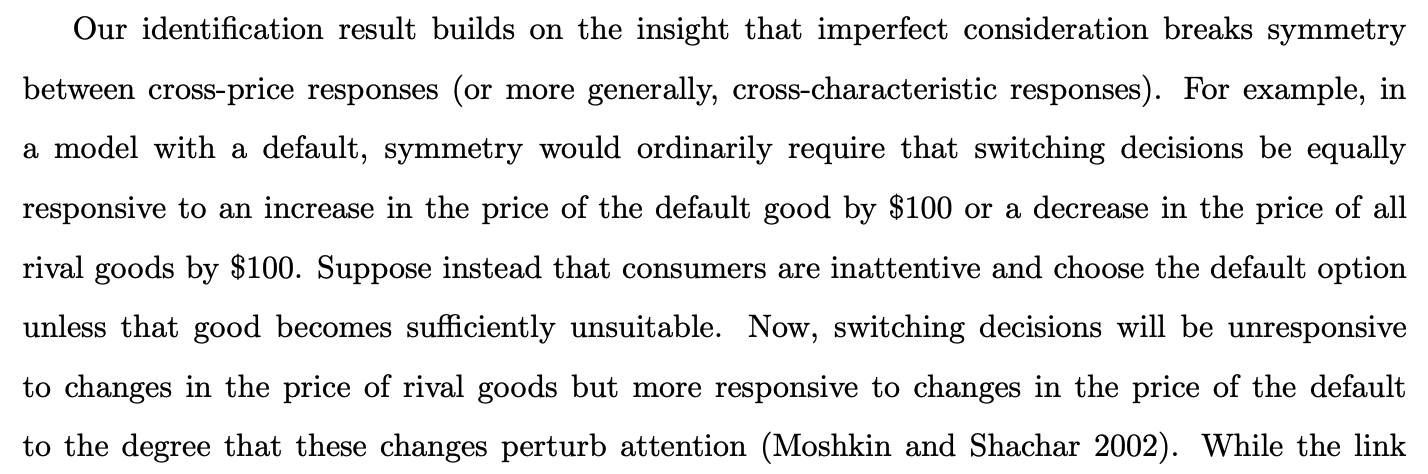
\includegraphics[width=\linewidth]{images/abaluck1.png}\\
%     %     ...
%     %     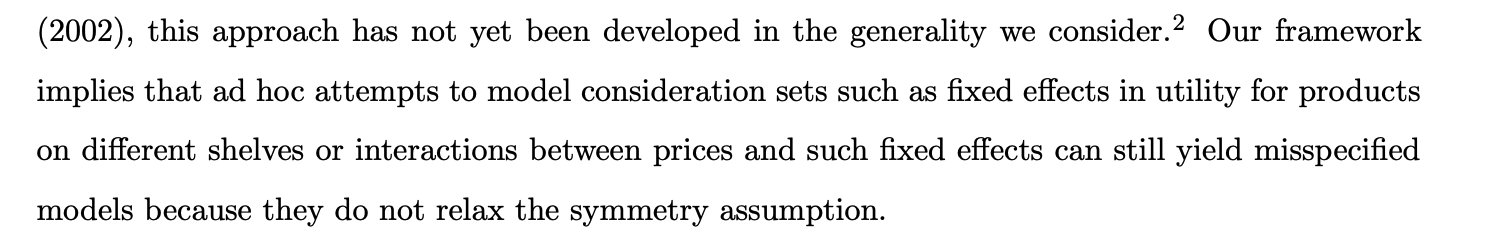
\includegraphics[width=\linewidth]{images/abaluck2.png}  
%     %   \end{center}
    

% Simple case considered in paper is when there is a base default that people focus on (and ignore other choices).
% Default Specific Model. More rich setting: Alternative Specific Choice model. Put structure on how a choice is selected into a consideration set. In both cases, can identify the consideration choice probabilities using price elasticities. This can be a very important thing to model if your counterfactual relates to changes in the consideration set.  However, it may not be first order to your problem at hand.
      
%       %%% UPDATE
%


          
      
% \subsection{Koijen and Yogo (2019)}
      
% Influential paper by Koijen and Yogo (2019) estimates a
%               demand system for financial assets. The framework is used to study the Distribution of price elasticities with respect to demand shocks (residual demand)and Decomposing variation in asset returns
              
% %               
\includegraphics[width=\linewidth]{images/koijenyogo.pdf}
% %  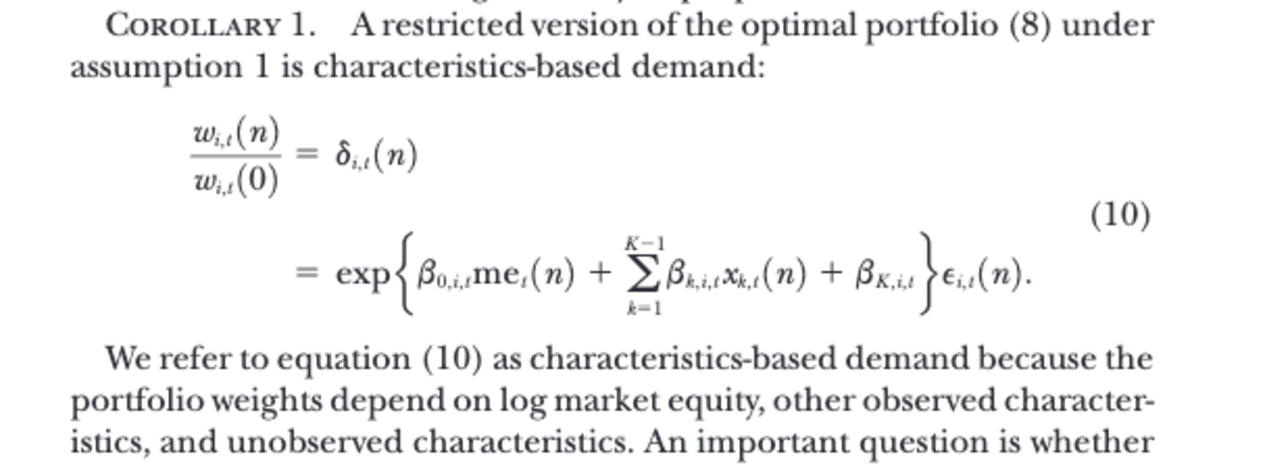
\includegraphics[width=\linewidth]{images/koijenyogo4.pdf}
% %  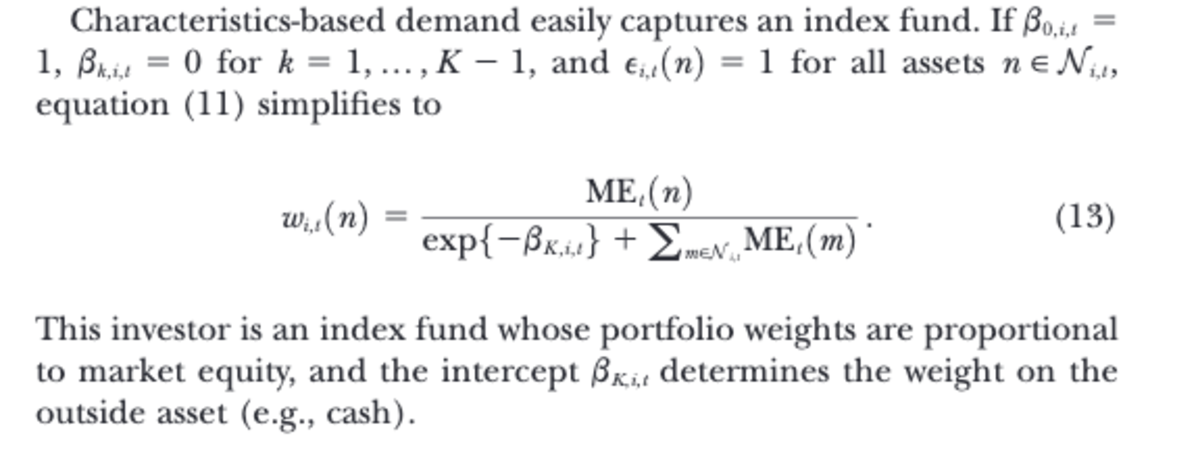
\includegraphics[width=\linewidth]{images/koijenyogo3.pdf}
% % 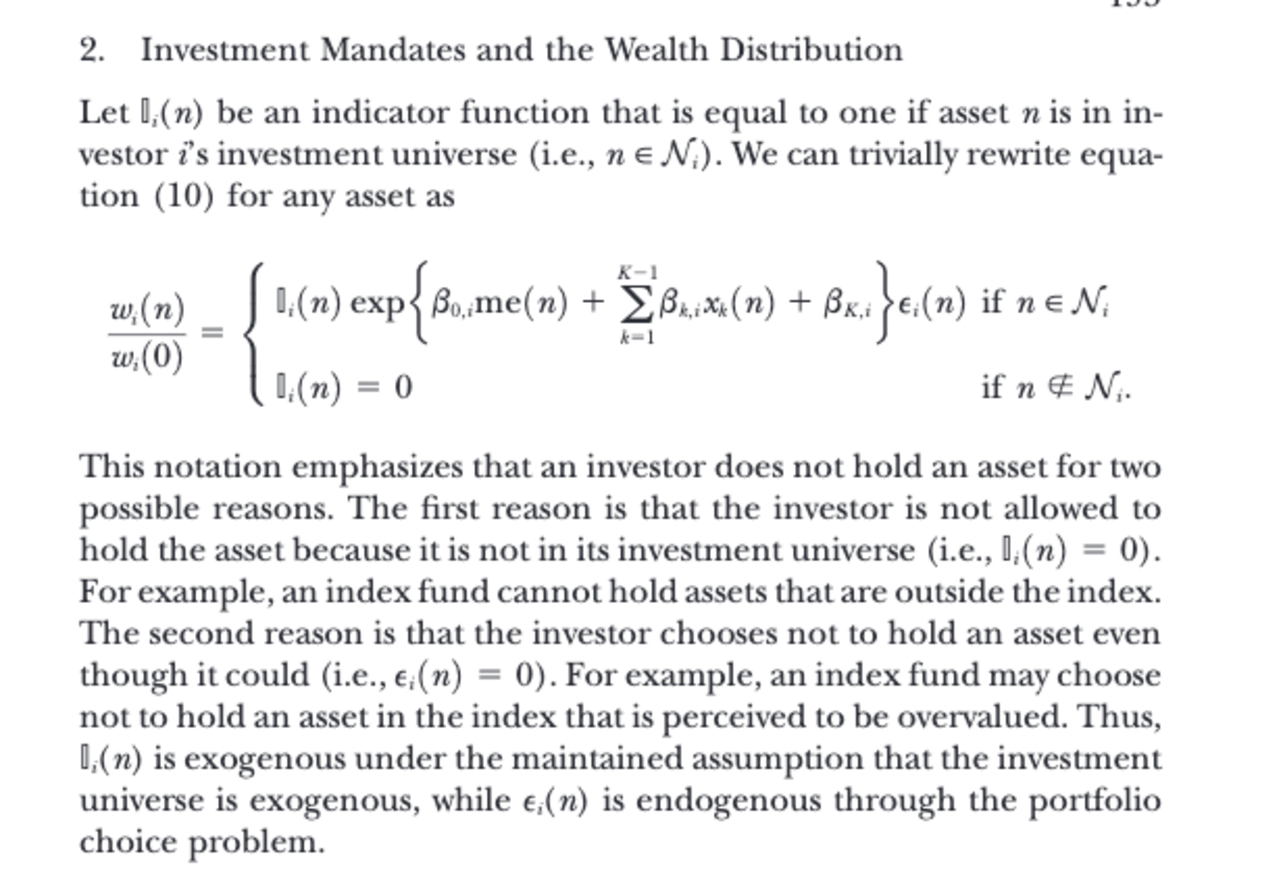
\includegraphics[width=\linewidth]{images/koijenyogo2.pdf}




\bibliography{lecture_note_bib.bib}
\bibliographystyle{plainnat}

\end{document}